% first of all, precise the document class: report, article, book, beamer, standalone, ...
% this has no effect on the vast majortiy, however, certain options or pagination are only available for certain types
\documentclass{article}


\usepackage[margin=1in]{geometry} % this will set the margins of the document to 1 inch on all sides. You can change this value to increase or decrease the margins.
\usepackage{graphicx} % allows to include images in the document using the command \includegraphics
\usepackage{hyperref} % enables clickable links and cross-references (\href, \url, \hyperref)
\usepackage{amsmath} % load the package amsmath to have access to advanced math functionalities
\usepackage{color} % color package allows to use colors in the document, for example for text or background. You can define your own colors using \definecolor, or use predefined colors such as red, blue, green, etc.

\newcommand{\Overleaf}{(PLACEHOLDER)}

% document metadata
% set the title of the document
\title{\LaTeX Introduction Course}
% set the author of the document
\author{Romain De Groote}
% set the date of the document (today allows to automatically insert the current date)
\date{\today}

\setcounter{tocdepth}{2} % this will allow to include subsections in the table of contents, but not subsubsections. You can change this value to include more or less levels of sections in the table of contents.

% This is where the content of the document starts
\begin{document}


\maketitle % generate the title using the metadata defined above

\newpage % this will start a new page, so that the title and the table of contents are on separate pages.

\tableofcontents % this will generate a table of contents based on the sections and subsections defined in the document

% create a new section called Introduction
\section{Introduction}

\LaTeX is a document preparation system and markup language widely used for the communication and publication of scientific documents in many fields, including mathematics, computer science, engineering, physics, chemistry, and economics. It provides a high-quality typesetting system that is particularly well-suited for documents containing complex mathematical equations and symbols.

\subsection{Easy to learn, easy to use}

\LaTeX is quite easy to learn and use, if you don't need a local installation the best option is clearly to use \Overleaf, a free online latex editor. It integrates a great project manager, allowing to share it to other user and provide a vast range of templates and tutorials for get started with \LaTeX.

For you to learn how to write a document in \LaTeX, a quick introduction is provided in this document. However, if you really want to be able to do everything you want with \LaTeX, there is no secret: you'll have to pass hours to search online, read questions on stackexchange, read the documentation of the packages you want to use, and so on. But don't worry, it's really worth it, and you'll be able to do things that are impossible to do with word.

\subsection{Why use \LaTeX?}

There is several reasons why Latex is widely used in academia and scientific publishing:
\begin{itemize}
  \item \textbf{Open-source and free:} \LaTeX is an open-source software, which means that it is freely available to anyone who wants to use it. 
  \item \textbf{High-quality typesetting:} \LaTeX produces high-quality documents with a professional look and feel. It is particularly well-suited for documents containing complex mathematical equations and symbols, as it provides a powerful set of tools for typesetting mathematics.
  \item \textbf{Customizability:} \LaTeX is highly customizable, allowing users to create their own document classes, packages, and styles. This makes it possible to create documents that are tailored to specific needs and requirements.
  \item \textbf{Cross-platform compatibility:} \LaTeX is available on multiple platforms, including Windows, Mac, and Linux. This makes it easy to collaborate with others who may be using different operating systems.
  \item \textbf{Large community and support:} \LaTeX has a large and active community of users and developers who contribute to the development of the software and provide support to other users. This means that there are many resources available online, including tutorials, forums, and documentation, to help users learn and use \LaTeX effectively.
  \item \textbf{Integration with other tools:} \LaTeX can be easily integrated with other tools and software, such as reference managers, version control systems, and collaborative writing platforms. This makes it a powerful tool for academic writing and publishing.
\end{itemize}

However, to be perfectly honest, one of the used \LaTeX editor and compiler, Overleaf, is not open-source, and a lot of its features are prenium.

\subsection{Overleaf}

Overleaf is a freenium online LaTeX editor that allows users to create, edit, and collaborate on LaTeX documents in real-time. It provides a clean UI for writing and editing LaTeX code, as well as a project manager. However, it's still an online tool, meaning that you need an internet connection to use it, and that you are dependent on the servers of Overleaf.
 % this will include the content of the file 1.Introduction.tex at this place, as if it was copy-pasted here. This allows to split the content of the document into several files, which is very useful for large documents. The path is relative to the main file, and the extension .tex is optional.

\section{Use}
\subsection{Online - Overleaf}

\subsubsection{Account Creation}

To use Overleaf, you need to create an account. You can sign up for a \href{https://www.overleaf.com/register}{free account} using your email address or by linking your Google account\footnote{Use your personnal email address to create the account, you can add school/professional email address later to benefit from additional features if you are elligible.}. Once you have created an account, you can start creating and editing LaTeX documents.

\subsection{New Project}

To create a new project in Overleaf, simply click on the "New Project" button on the dashboard.

You will then be prompted to choose a template for your project. In addition to the basic templates, you can also find a wide range of templates for different types of documents, such as academic papers, presentations, posters, and more. You can also start with a blank project if you prefer to write your LaTeX code from scratch.

As said in the introduction, Overleaf is a freenium tool, however it has successfully implemented itself despite it, how? This can be explain by different factors:
\begin{itemize} 
  \item \textbf{Ease of use:} Overleaf UI is very user-friendly and intuitive, in addition coloborate with it is really easy.
  \item \textbf{Agreement with institutions:} A lot of universities and research institutions have agreements with Overleaf, offering to their students and researchers free access to the premium features of Overleaf.
  \item \textbf{Vast range of templates:} The community of Overleaf is very active, and a lot of templates are available for free, which can be a great incentive for users to use Overleaf.
  \item \textbf{Documentation:} Overleaf provides a vast range of documentation and tutorials to do everything you want with LaTeX, which can be a great incentive for users to use Overleaf.
\end{itemize}

\subsubsection{Counterpart...}

There is 2 main counterparts I could find:
\begin{itemize}
  \item \textbf{Dependence on the prenium features:} Some prenium features of Overleaf are most than useful, and downgrading from a prenium account to a free account can be really frustrating, especially if you have the habit to use these features.
  \item \textbf{Dependence on the servers of Overleaf:} To be clear, Overleaf is a really good tool, and its servers are really reliable, but you are still dependent on them.\newline
  {\color{blue} %change the color of the text to blue in its scope, the {...} around the text limit the scope of the color change.
    May the 14th 2025, Overleaf servers were down for more than 6 hours, a lot of users were really frustrated, some panicked because of their deadlines, and in all this chaos, a lot of user were the happy ones, because they had the habit to have a local backup of their projects. To add to this, this was the day before the dealine for the NeurIPS 2025 and some Master thesis.
  }\newline
  The moral of this is: always have numerous backups of your sensitive projects.
\end{itemize}

The big issue, is that Git, Github and Dropbox are prenium features of Overleaf.

\subsection{Offline - TeXLive}

If you want to use LaTeX offline, you can download a local distribution of LaTeX such as TeX Live. This will allow you to compile LaTeX documents on your own computer without needing an internet connection.

It is then possible to use a local LaTeX editor such as TeXworks, TeXstudio, or VSCode with the LaTeX Workshop extension. These editors provide a user-friendly interface for writing and editing LaTeX code, as well as features such as syntax highlighting, code completion, and error checking.


\subsection{Offline Overleaf free}

To have access to an offline version of an Overleaf project, you can follow these steps:
\begin{itemize}
  \item Install Vs Code
  \item Install the Overleaf Workshop extension
  \item Install LaTeX Workshop extension
  \item Remote access to the Overleaf project using the Overleaf Workshop extension, which will allow you to edit your Overleaf project in VSCode
  \item Create a local version of the project (be aware, this is still real time editing and losing the connection and then reconnecting will cause the local version to be updated with the online version, which can cause loss of work if you have made changes in the local version while being disconnected)
  \item Init Git
  \item Create a new branch for the local version
  \item cut your internet connection, and work on the local version
  \item Checkout to main branch, and reconnect to the internet, which will update the local version with the online version
  \item Merge the local branch with the main branch, which will allow you to keep your changes and update the online version with them
\end{itemize}


\section{Writting}

LaTeX is a markup language, meaning that you write your document using commands and syntax that describe the structure and formatting of the document, rather than directly manipulating the visual appearance of the document as you would in a word processor. This allows for greater control and flexibility over the formatting of the document, but it also means that there is a learning curve to using LaTeX effectively.

In LaTeX, there is 2 main types of macros: commands and environments. Commands are used to perform specific actions, such as formatting text, inserting images, or creating tables. Environments are used to define a block of content that has a specific formatting or behavior, such as a section, a figure, or a table.

\subsection{Preamble}

The preamble of a \LaTeX document is the section that comes before the \texttt{\(\backslash\)begin\{document\}} command, and it is used to define the document class, load packages, and set up any custom commands or configurations for the document. The preamble is an important part of a \LaTeX document, as it allows you to customize the behavior and appearance of your document, and it can also help to ensure that your document is properly formatted and structured.

\subsection{Document management}

To structure your document, you can use sections, subsections, ... They follow this order:
  \begin{itemize}
    \item \texttt{\(\backslash\)part\{...\}} for parts
    \item \texttt{\(\backslash\)chapter\{...\}} for chapters (only in book and report document classes)
    \item \texttt{\(\backslash\)section\{...\}} for sections
    \item \texttt{\(\backslash\)subsection\{...\}} for subsections
    \item \texttt{\(\backslash\)subsubsection\{...\}} for subsubsections
    \item \texttt{\(\backslash\)paragraph\{...\}} for paragraphs
    \item \texttt{\(\backslash\)subparagraph\{...\}} for subparagraphs
  \end{itemize}

In addition, if you manage a multiple files document, you can use the \texttt{\(\backslash\)include} or \texttt{\(\backslash\)input} command to include the content of other files in your main document. The \texttt{\(\backslash\)include} command is used to include a file that contains a complete section or chapter of the document, while the \texttt{\(\backslash\)input} command is used to include a file that contains a smaller piece of content, such as a figure or a table. Both commands allow you to organize your document into multiple files, which can make it easier to manage and edit large documents.

\subsection{Text mode}

In text mode, you can write normal text, and use commands to format it. For example, the \texttt{\(\backslash\)textbf} command is used to make text bold, and the \texttt{\(\backslash\)emph} command is used to emphasize text (usually by italicizing it). You can also use commands to change the font size, color, or style of the text. The text mode is the default mode in LaTeX, and it is used for writing the main content of the document.

\subsection{Math mode}

In math mode, you can write mathematical expressions using a special syntax. For example, the \texttt{\(\backslash\)frac} command is used to create a fraction, and the \texttt{\(\backslash\)sum} command is used to create a summation symbol. Math mode also allows you to use special symbols and characters that are not available in text mode, such as Greek letters, operators, and delimiters. To enter math mode, you can use \texttt{\(\backslash\)(} and \texttt{\(\backslash\))} for inline math, or \texttt{\(\backslash\)[\(\backslash\)]} for display math, which is centered and on its own line.

\subsection{Commands}

Commands in LaTeX are defined using a backslash followed by the name of the command, and they can take arguments that specify the content or formatting of the command. For example, the \texttt{\(\backslash\)LaTeX} command is used to generate the LaTeX logo. Be aware that command can be mode specific, meaning that they can only be used in certain contexts or environments. For example, the \texttt{\(\backslash\)alpha} command is used to display the \(\alpha\) symbol, but it can only be used in math mode, which is a special environment for writing mathematical expressions.

\subsection{Environments}
Environments in LaTeX are defined using the \texttt{\(\backslash\)begin} and \texttt{\(\backslash\)end} commands, and they can also take arguments that specify the content or formatting of the environment. For example, the \texttt{itemize} environment is used to create a bulleted list, and it is defined as follows:
\begin{verbatim}
\begin{itemize}
  \item First item
  \item Second item
  \item Third item
  \item Fourth item
\end{itemize}
\end{verbatim}
This will generate a bulleted list with four items. The \texttt{itemize} environment can also be nested inside other environments, such as a section or a figure, to create more complex documents.

There is also math specific environments, such as the \texttt{equation} environment, which is used to create numbered equations, and the \texttt{align} environment, which is used to align multiple equations. These environments allow you to write complex mathematical expressions in a clear and organized way. Those enviroments are numbered by default, but you can add a \texttt{*} at the end of the environment name to create an unnumbered version of the environment, for example \texttt{equation*} and \texttt{align*}.

\subsection{Figure and tables}

Figure are also defined as environments, using the \texttt{figure} environment. Inside the figure environment, you can use the \texttt{\(\backslash\)includegraphics} command to include an image file, and you can also add a caption and a label to the figure for referencing it later in the document. For example:
\begin{verbatim}
\begin{figure}
  \centering
  \includegraphics[width=0.5\textwidth]{example-image}
  \caption{An example image}
  \label{fig:example}
\end{figure}
\end{verbatim}

Table are for their part defined using the \texttt{table} environment, and they can be created using the \texttt{tabular} environment inside the table environment. The \texttt{tabular} environment allows you to define the structure of the table, such as the number of columns and their alignment, and you can also add a caption and a label to the table for referencing it later in the document. For example:
\begin{verbatim}
\begin{table}
  \centering
  \begin{tabular}{|c|c|c|}
    \hline
    Column 1 & Column 2 & Column 3 \\
    \hline
    Data 1 & Data 2 & Data 3 \\
    Data 4 & Data 5 & Data 6 \\
    \hline
  \end{tabular}
  \caption{An example table}
  \label{tab:example}
\end{table}
\end{verbatim}
This will generate a table with three columns and two rows of data, with a caption and a label for referencing it later in the document. You can also customize the appearance of the table using various commands and packages, such as \texttt{booktabs} for creating professional-looking tables, or \texttt{tabularx} for creating tables with adjustable column widths. Math mode has also its own table environment, called \texttt{array}, which allows you to create tables with mathematical content, such as matrices or systems of equations. The syntax for the \texttt{array} environment is similar to the \texttt{tabular} environment, but it is designed specifically for mathematical content.

\subsection{Bibliography}

You can create a bibliography in LaTeX using the \texttt{thebibliography} environment, which allows you to list your references and cite them in the document. Inside the \texttt{thebibliography} environment, you can use the \texttt{\(\backslash\)bibitem} command to define each reference, and you can also use the \texttt{\(\backslash\)cite} command to cite the references in the text. For example:
\begin{verbatim}
\begin{thebibliography}{9}
  \bibitem{knuth} Donald E. Knuth. \textit{The TeXbook}. Addison-Wesley, 1984.
\end{thebibliography}
\cite{knuth}
\end{verbatim}

Or if you want you can use BibTeX or BibLaTeX, which are tools for managing bibliographies in LaTeX. They allow you to create a separate bibliography file (with a .bib extension) that contains all your references, and then you can use the \texttt{\(\backslash\)bibliography} command to include the bibliography in your document. This can make it easier to manage your references, especially if you have a large number of them, and it also allows you to easily switch between different citation styles using the \texttt{\(\backslash\)bibliographystyle} command.

\subsection{Cross-referencing}

You can create a cross-reference in LaTeX using the \texttt{\(\backslash\)label} and \texttt{\(\backslash\)ref} commands. The \texttt{\(\backslash\)label} command is used to define a label for a specific element in the document, such as a section, a figure, or a table, and the \texttt{\(\backslash\)ref} command is used to reference that label later in the document.

\subsection{Create figure and graphes}

The Tikz package is a powerful tool for creating high-quality graphics and diagrams in LaTeX. It allows you to create complex figures and graphs using a simple and intuitive syntax, and it provides a wide range of options for customizing the appearance of your graphics. With Tikz, you can create everything from simple shapes and lines to complex diagrams and plots, making it a versatile tool for creating visual content in your LaTeX documents.

For example, the following code draws two axes, a parabola and a point on it, and gives the Figure~\ref{fig:tikz}. This code is written in the file \texttt{src/TikZExample.tex}, which is used twice: once displayed as code with \texttt{\(\backslash\)verbatiminput}, and once compiled with \texttt{\(\backslash\)input}, so the figure always matches the code.
\verbatiminput{./../src/TikZExample.tex} % display the code of the file
\begin{figure}[h]
  \centering
  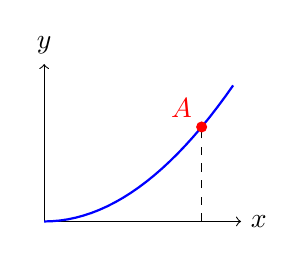
\begin{tikzpicture}
  \draw[->] (0,0) -- (2.5,0) node[right] {$x$};
  \draw[->] (0,0) -- (0,2) node[above] {$y$};
  \draw[blue, thick, domain=0:2.4]
    plot (\x, {0.3*\x*\x});
  \draw[dashed] (2,0) -- (2,1.2);
  \fill[red] (2,1.2) circle (2pt)
    node[above left] {$A$};
\end{tikzpicture}
 % compile the same file
  \caption{A simple TikZ drawing}
  \label{fig:tikz}
\end{figure}

\subsection{Create your own commands and environments}

You can create your own commands and environments in LaTeX using the \texttt{\(\backslash\)newcommand} and \texttt{\(\backslash\)newenvironment} commands. The \texttt{\(\backslash\)newcommand} command allows you to define a new command that can be used throughout your document, while the \texttt{\(\backslash\)newenvironment} command allows you to define a new environment that can be used to structure your document in a specific way. Creating your own commands and environments can help to simplify your document and make it easier to read and maintain, especially if you have complex formatting or repetitive content in your document. For example:
\begin{verbatim}
\newcommand{\R}{\mathbb{R}} % this will create a new command \R that will display the symbol for the set of real numbers
\newenvironment{myenv}{\begin{center}}{\end{center}} % this will create a new environment called myenv that will center the content inside it
\end{verbatim}

However, if you need to create more complex commands or environments, the \texttt{\(\backslash\)newcommand} and \texttt{\(\backslash\)newenvironment} commands may not be sufficient, and hard to use due on how they handle optional arguments. In this case, you can use the \texttt{\(\backslash\)NewDocumentCommand} and \texttt{\(\backslash\)NewDocumentEnvironment} commands from the \texttt{xparse} package, which provide more advanced features for creating custom commands and environments, such as support for optional arguments and more flexible syntax.


\section*{Conclusion} % the * in \section* means that this section will not be numbered, and will not appear in the table of contents. You can use this for sections that are not part of the main structure of the document, such as an introduction or a conclusion.

In conclusion, LaTeX is a powerful and flexible typesetting system that allows you to create professional-looking documents with precise control over formatting and structure. Whether you are writing a simple report or a complex book, LaTeX provides the tools and features necessary to produce high-quality output. With its extensive package ecosystem and active community, LaTeX continues to be a popular choice for academics, researchers, and professionals across various fields. By mastering LaTeX, you can enhance your document creation skills and produce polished, well-structured documents with ease. Overleaf, the main LaTeX editor, provides a user-friendly interface and collaborative features that make it easier than ever to create and share LaTeX documents. Whether you are new to LaTeX or an experienced user, Overleaf offers a convenient platform to write, edit, and compile your LaTeX projects efficiently. However, the free plan can be limiting, and relying only on online editors can be risky, so try to always have a local backup of your work with a local installation to work with in case.\newline
If I can ask give a final advise, as always, practice is key to mastering LaTeX. The more you use it, the more comfortable you will become with its syntax and features.

\end{document}
% this is where the content of the document ends